\chapter{PC Program}
\label{chap:pc_program}
A PC program will show the position of the hit point and the hight the ball will bounce back to.

\section{Communication and Logic}
\label{subsec:pc_program_com}
Regarding the communication, the PC program and the FPGA are connected by a USB wire and this protocol is handle by the qt serial libraries given. This let the communication in hands of a code that has been already tested.

In respect of the logic behind the PC program, the PC ask to the FPGA if a new brick has been detected, if so, ask for the color of the new brick. This is implemented thanks to two registers in the FPGA, one for the $new brick$ that turns true when a new brick is detected, and another for the $color$ where the values of the brick's color is saved.

Also, the detection thresholds of the new brick can be change from the PC interface so the FPGA hasn't had to be reconfigured.  

\section{Interface}
\label{subsec:pc_program_interface}
The main reason to implement a UI is the easy to introduce the new values for calibration. Due to the system is portable and the environment changeable, the system require of some values to be modifiable in order to calibrate it. In this case there are two factors to modify: the refresh and the thresholds. 

On one hand, the refresh determines when the PC program ask to the FPGA for a new brick. A higher value will decrease the total power consumption while it could mean that, if a new brick appears before the order was sent, a new brick can be lost by the PC program.

On the other hand, the thresholds for each brick need to be calibrated depending on the ambient conditions. Despite the fact probably this only need to be made once, due to the fact the system is under controlled conditions, an easy calibration system has been implemented as shows the figure \ref{fig:UI_settings}.

	\begin{figure}[!ht]
		\centering
		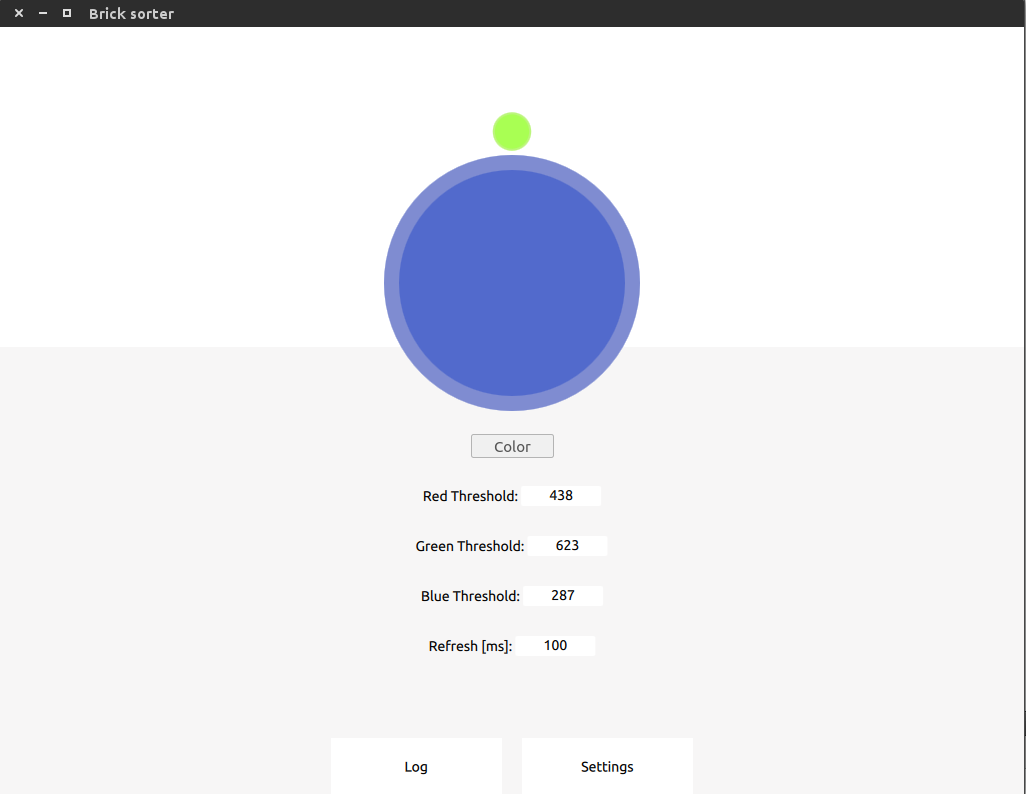
\includegraphics[width=.7\textwidth]{figures/UI_settings}
		\caption{PC program implemented with Qt. Detail of Settings tab.}
		\label{fig:UI_settings}
	\end{figure}

Furthermore, the PC program has a data log where relevant information of the FPGA is shown. The UI also shows the last brick detected by the machine and shows a graphical history in form of smaller circles as can be seen in the figure \ref{fig:UI_log}.

	\begin{figure}[!ht]
		\centering
		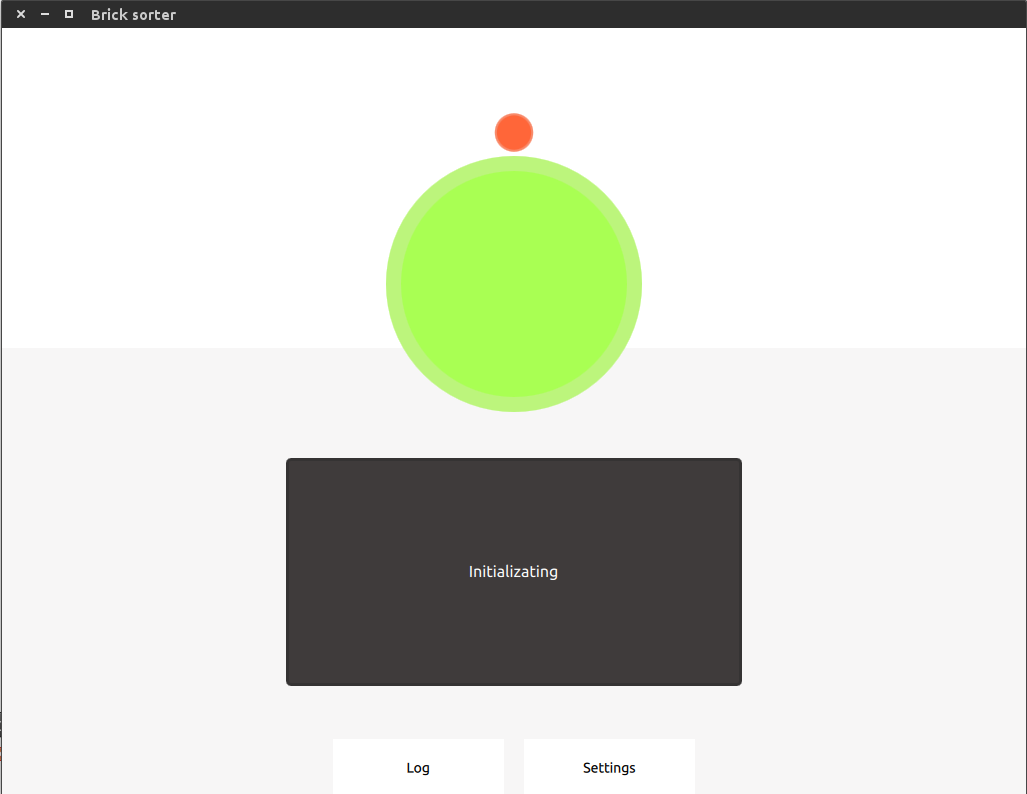
\includegraphics[width=.7\textwidth]{figures/UI_log}
		\caption{PC program implemented with Qt. Detail of Log tab.}
		\label{fig:UI_log}
	\end{figure}

	